\chapter{向量与空间解析几何}
\section{向量及其基本运算}
\subsection{向量的概念}
\defination[向量的定义]
\noindent
\begin{minipage}{0.6\linewidth}
\hspace*{2em} 既有大小也有方向的量称为\highlight{dy}{\index{XL@向量}向量}(或\highlight{dy}{\index{SL@矢量}矢量})。通常我们用有向线段来表示向量。\\
\hspace*{2em} 以$A$为\highlight{dy}{\index{QSD@起始点}起始点}、$B$为\highlight{dy}{\index{ZD@终点}终点}的有向线段所表示的向量记为$\boldsymbol{AB}$.有时也会用一个黑体字母来表示向量。例如$\boldsymbol{a}$,$\boldsymbol{b}$.向量$\boldsymbol{AB}$的长度表示\highlight{dy}{\index{XLDDX@向量的大小}向量的大小},记作\highlight{dy}{\index{XLDM@向量的模}向量的模}。\\
\hspace*{2em} 向量的四要素:起始点、终点、方向、模。
\end{minipage}
\begin{minipage}{0.4\linewidth}
	\centering
	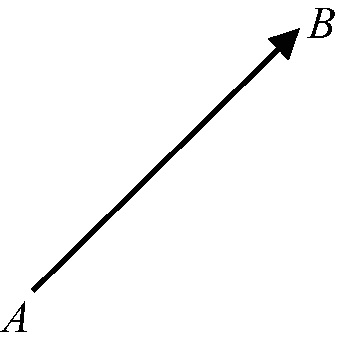
\includegraphics[width = 0.45\linewidth]{pic/C-5/vec}
	\vspace*{-1em}
	\captionof{figure}{向量示意图}
	\label{向量示意图}
\end{minipage}

\defination[自由向量的定义]
在实际研究中,我们只关心向量的方向和大小,称为\highlight{dy}{\index{ZYXL@自由向量}自由向量}。\\

\vspace*{-1em}
\defination[向量的夹角定义]

\noindent
\begin{minipage}{0.5\linewidth}
\hspace*{2em} 设有两个非零向量$\boldsymbol{a}$,$\boldsymbol{b}$,任取空间中一点$O$,作$\boldsymbol{OA}=\boldsymbol{a}$,$\boldsymbol{OB}=\boldsymbol{b}$,规定$0\leq \varphi=\angle AOB\leq \pi$,那么$\angle AOB$称为\highlight{dy}{\index{XLDJJ@向量的夹角}向量$\boldsymbol{a}$,$\boldsymbol{b}$的夹角},记作$\langle\boldsymbol{a}$,$\boldsymbol{b}\rangle$或$\langle\boldsymbol{b}$,$\boldsymbol{a}\rangle$,即$\langle\boldsymbol{a}$,$\boldsymbol{b}\rangle=\varphi$.\\
\hspace*{2em} 特别地,如果$\langle\boldsymbol{a}$,$\boldsymbol{b}\rangle=0$或$\pi$,就称向量$\langle\boldsymbol{a},\boldsymbol{b}
\rangle$平行记作$\boldsymbol{a}\parallel\boldsymbol{b}$,当$\boldsymbol{a}$,$\boldsymbol{b}$平移至起点相同的时候,那么$\langle\boldsymbol{a}$,$\boldsymbol{b}\rangle$一定共线。所以,两个平行的向量也称为\highlight{dy}{\index{GXXL@共线向量}共线向量}。\\
\hspace*{2em} 如果$\langle\boldsymbol{a}$,$\boldsymbol{b}\rangle$=$\di\frac{\pi}{2}$,就称向量$\boldsymbol{a}$,$\boldsymbol{b}$垂直,记作$\boldsymbol{a}\perp\boldsymbol{b}$.
\end{minipage}
\begin{minipage}{0.5\linewidth}
	\centering
	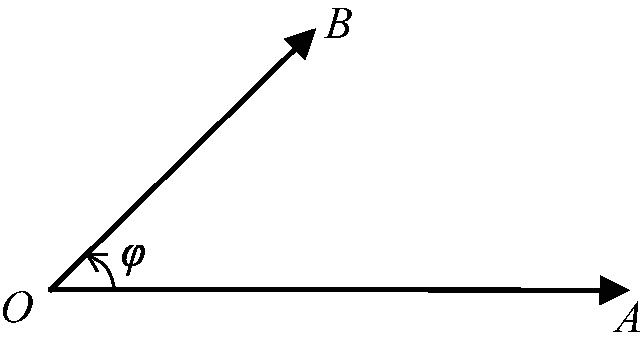
\includegraphics[width = 0.6\linewidth]{pic/C-5/vecang}
	\vspace*{-1em}
	\captionof{figure}{向量的夹角}
	\label{向量的夹角}
\end{minipage}

\warn[\par 零向量与另外的向量的夹角可以任意在{[0,$\pi$]}中取值。因此,可以认为零向量与任何向量都平行(垂直)]
\defination[向量相等的定义]
如果两个向量$\boldsymbol{a}$,$\boldsymbol{b}$大小和方向都相同,那么向量$\boldsymbol{a}$,$\boldsymbol{b}$是相等的,记作$\boldsymbol{a}=\boldsymbol{b}$.\\

\vspace*{-1em}
\defination[零向量的定义]
零向量的模长为0,方向可以为任意方向。用$\boldsymbol{0}$或者$\vec{0}$表示。
\subsection{向量的线性运算}
向量的线性运算分为加法运算、减法运算以及数乘运算。
\\ 1.$\,$加法运算法则\\

\vspace*{-1em}\vspace*{-1em}
\defination[向量的加法]
平行移动使向量$\boldsymbol{a},\boldsymbol{b}$有共同起点,然后由\highlight{dy}{\index{PXSBXFZ@平行四边形法则}平行四边形法则},以$\boldsymbol{a},\boldsymbol{b}$为相邻两边作平行四边形,将平行四边形的对角线所形成的向量定义为\highlight{dy}{\index{HXL@和向量}和向量}。
\par 或者由\highlight{dy}{\index{SJXFZ@三角形法则}三角形法则},将$\boldsymbol{b}$的起点移至$\boldsymbol{a}$的终点(即首尾相连),然后和向量为$\boldsymbol{a}$的起点指向$\boldsymbol{b}$的终点。
\begin{figure}[h]
\begin{minipage}{0.5\linewidth}
	\centering
	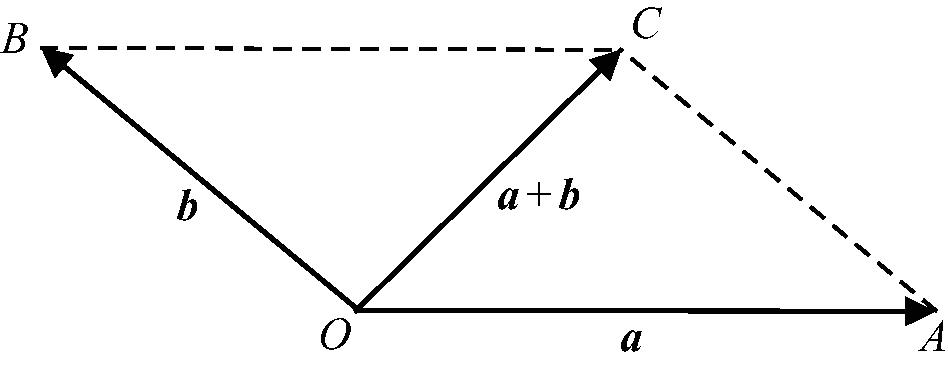
\includegraphics[width = 0.81\linewidth]{pic/C-5/vecadd}
\end{minipage}
\begin{minipage}{0.5\linewidth}
	\centering
	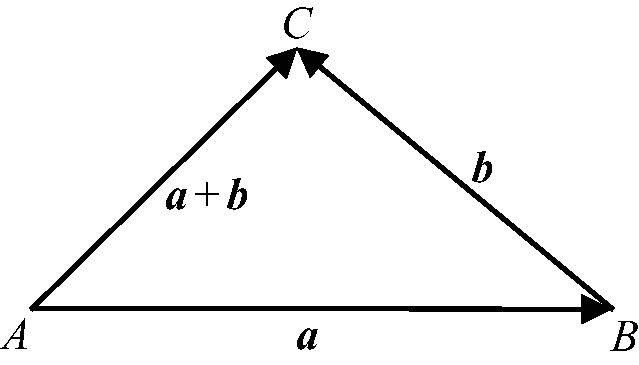
\includegraphics[width = 0.57\linewidth]{pic/C-5/vecadd2}
\end{minipage}
\caption{向量的加法}
\label{向量的加法}
\end{figure}

\begin{minipage}{0.5\linewidth}
\noindent \textbf{加法的运算规律:}\\
(1)$\,$ \highlight{dy}{\index{JFJHL@加法交换律}加法交换律} \qquad $\boldsymbol{a}+\boldsymbol{b}=\boldsymbol{b}+\boldsymbol{a} $\\
(2)$\,$ \highlight{dy}{\index{JFJHL@加法结合律}加法结合律} \qquad ($\boldsymbol{a}+\boldsymbol{b})+\boldsymbol{c}=\boldsymbol{a}+(\boldsymbol{b}+\boldsymbol{c}) $\\
\end{minipage}
\begin{minipage}{0.5\linewidth}
	\centering
	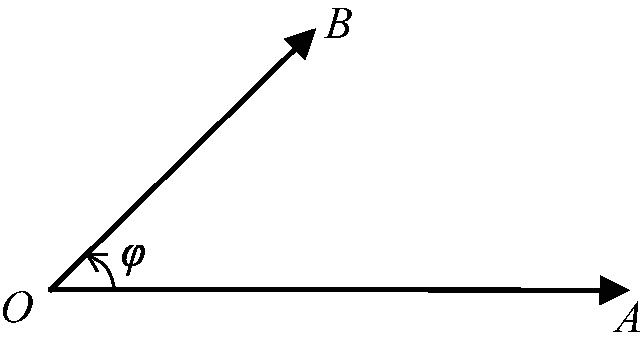
\includegraphics[width = 0.5\linewidth]{pic/C-5/vecang}
	\vspace*{-1em}
	\captionof{figure}{向量的加法运算规律}
	\label{向量的加法运算规律}
\end{minipage}

\noindent 2.$\,$减法运算法则\\
\vspace*{-1em}\vspace*{-1em}

\defination[向量的差定义]
与向量$\boldsymbol{a}$模长相同而方向相反的向量叫做$\boldsymbol{a}$的\highlight{dy}{\index{FXL@反向量}反向量},记作$-\boldsymbol{a}$,那么\highlight{dy}{\index{XLDC@向量的差}向量$\boldsymbol{b},\boldsymbol{a}$的差}为:
\begin{equation}
	\boldsymbol{b}-\boldsymbol{a}=\boldsymbol{b}+(-\boldsymbol{a})
\end{equation}
可以理解为把向量$-\boldsymbol{a}$加到向量$\boldsymbol{b}$上。(即理解为加法运算的逆运算,其运算满足加法运算的所有规律)

\begin{figure}[h]
	\begin{minipage}{0.5\linewidth}
		\centering
		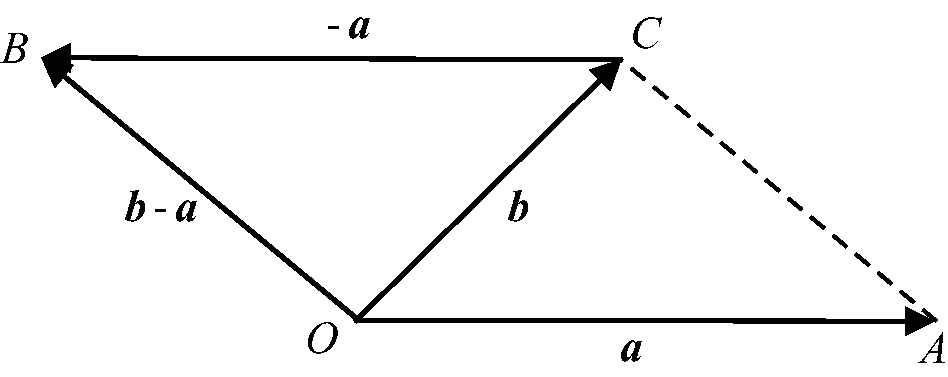
\includegraphics[width = 0.81\linewidth]{pic/C-5/vecdel}
	\end{minipage}
	\begin{minipage}{0.5\linewidth}
		\centering
		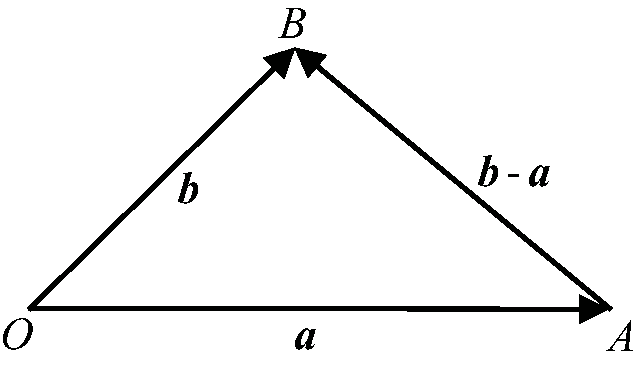
\includegraphics[width = 0.57\linewidth]{pic/C-5/vecdel2}
	\end{minipage}
	\caption{向量的减法}
	\label{向量的减法}
\end{figure}

\noindent 3.$\,$数乘运算法则\\

\vspace*{-1em} \vspace*{-1em}
\defination[向量的数乘定义]
向量$\boldsymbol{a}$与实数$\lambda$的乘积记作$\lambda\boldsymbol{a}$,规定$\lambda\boldsymbol{a}$也是一个向量,它的模
\begin{equation}
	|\lambda\boldsymbol{a}|=|\lambda||\boldsymbol{a}|
\end{equation}
它的方向有三种情况:\\
(1)$\,$ 当$\lambda>0$时,其方向与$\boldsymbol{a}$相同;\\
(2)$\,$ 当$\lambda<0$时,其方向与$\boldsymbol{a}$相反;\\
(3)$\,$ 当$\lambda=0$时,$\lambda\boldsymbol{a}$为零向量,这时其方向可以是任意的。\\
\textbf{数乘的运算规律:}\\
(1)$\,$ \highlight{dy}{\index{SCJHL@数乘交换律}数乘结合律} \qquad
$\lambda(\mu\boldsymbol{a})=\mu(\lambda\boldsymbol{a})=(\lambda\mu)\boldsymbol{a}$\\
(2)$\,$ \highlight{dy}{\index{SCFPL@数乘分配律}数乘分配律} \qquad
$(\lambda+\mu)\boldsymbol{a}=\lambda\boldsymbol{a}+\mu \boldsymbol{a}$\qquad $\lambda(\boldsymbol{a}+\boldsymbol{b})=\lambda\boldsymbol{a}+\lambda\boldsymbol{b}$
\subsection{向量的内积、外积及混合积}
\noindent1.$\,$向量的内积\\

\vspace*{-1em}\vspace*{-1em}
\defination[向量的内积定义]
向量$\boldsymbol{a},\boldsymbol{b}$的内积为
\begin{equation}
	\boldsymbol{a}\cdot\boldsymbol{b}=|\boldsymbol{a}||\boldsymbol{b}|\cos\langle\boldsymbol{a},\boldsymbol{b}\rangle
\end{equation}
特别地,当向量$\boldsymbol{a},\boldsymbol{b}$中有一个为零向量,其内积为0.向量的\highlight{dy}{\index{NJ@内积}内积}也称为\highlight{dy}{\index{SLJ@数量积}数量积}或\highlight{dy}{\index{DC@点乘}点乘}。\\
\textbf{点乘的运算规律:}\\
(1)$\,$\highlight{dy}{\index{JHL@交换律}交换律}\qquad $\boldsymbol{a}\cdot\boldsymbol{b}=\boldsymbol{b}\cdot\boldsymbol{a}$\\
(2)$\,$\highlight{dy}{\index{YSCDJHL@与数乘的结合律}与数乘的结合律}\qquad
$(\lambda\boldsymbol{a})\cdot\boldsymbol{b}=\lambda(\boldsymbol{a}\cdot\boldsymbol{b})$\\
(3)$\,$\highlight{dy}{\index{FPL@分配律}分配律}\qquad
$(\boldsymbol{a}+\boldsymbol{b})\cdot\boldsymbol{c}=\boldsymbol{a}\cdot\boldsymbol{c}+\boldsymbol{b}\cdot\boldsymbol{c}$\\
\textbf{内积的重要应用:}
\begin{equation}
	\boldsymbol{a}\perp\boldsymbol{b}\Leftrightarrow \boldsymbol{a}\cdot\boldsymbol{b}=0 
\end{equation}
2.$\,$向量的外积\\

\vspace*{-1em}\vspace*{-1em}
\defination[向量的外积定义]
向量$\boldsymbol{a}$,$\boldsymbol{b}$的外积$\boldsymbol{c}$为
\begin{equation}
	|\boldsymbol{c}|=|\boldsymbol{a}\times\boldsymbol{b}|=|\boldsymbol{a}||\boldsymbol{b}|\sin\langle\boldsymbol{a},\boldsymbol{b}\rangle
\end{equation}
其中外积$\boldsymbol{c}$的方向根据右手法则确定,就是手掌立在$\boldsymbol{a}$,$\boldsymbol{b}$所在平面的向量$\boldsymbol{a}$上,掌心向$\boldsymbol{b}$,那么大拇指方向就是垂直于该平面的方向,即为外积的方向。向量的\highlight{dy}{\index{WJ@外积}外积}也称为\highlight{dy}{\index{XLJ@向量积}向量积}或\highlight{dy}{\index{XLDCC@向量的叉乘}向量的叉乘}。\\

\noindent
\begin{minipage}{0.5\linewidth}
\textbf{外积的几何意义:}
\begin{equation}
	|\boldsymbol{a}\times\boldsymbol{b}|=|\boldsymbol{a}||\boldsymbol{b}|\sin \theta
\end{equation}
其中,$|\boldsymbol{a}\times\boldsymbol{b}|$是以$|\boldsymbol{a}|,|\boldsymbol{b}|$为邻边的平行四边形面积。\\
\textbf{外积的运算规律:}\\
(1)$\,$\highlight{dy}{\index{FJHL@交换律}反交换律}\qquad $\boldsymbol{a}\times\boldsymbol{b}=\boldsymbol{b}\times\boldsymbol{a}$\\
(2)$\,$\highlight{dy}{\index{FPL@分配律}分配律}\qquad
$(\boldsymbol{a}+\boldsymbol{b})\times\boldsymbol{c}=\boldsymbol{a}\times\boldsymbol{c}+\boldsymbol{b}\times\boldsymbol{c}$\\
(3)$\,$\highlight{dy}{\index{YSCDJHL@与数乘的结合律}与数乘的结合律}\qquad
$(\lambda\boldsymbol{a})\times\boldsymbol{b}=\boldsymbol{a}\times(\lambda\boldsymbol{b})=\lambda(\boldsymbol{a}\times\boldsymbol{b})$\\
\end{minipage}
\begin{minipage}{0.5\linewidth}
	\centering
	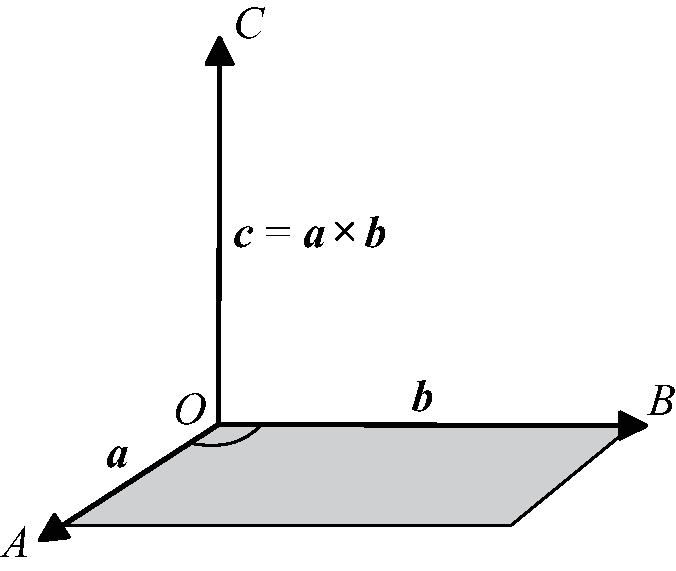
\includegraphics[width = 0.6\linewidth]{pic/C-5/veccross}
	\vspace*{-1em}
	\captionof{figure}{向量的外积}
	\label{向量的外积}
\end{minipage}

\noindent \textbf{外积的重要应用:}
\begin{equation}
	\boldsymbol{a}\parallel\boldsymbol{b}\Leftrightarrow \boldsymbol{a}\times\boldsymbol{b}=0
\end{equation}
3.$\,$向量的混合积\\

\vspace*{-1em}\vspace*{-1em}
\defination[向量混合积的定义] 

\noindent
\begin{minipage}{0.6\linewidth}
\hspace*{2em}设已知三个向量$\boldsymbol{a}$,$\boldsymbol{b}$,$\boldsymbol{c}$,数量$(\boldsymbol{a}\times\boldsymbol{b})\cdot \boldsymbol{c}$称为这三个向量的\highlight{dy}{\index{HHJ@混合积}混合积},记为$[\boldsymbol{a}\,\boldsymbol{b}\,\boldsymbol{c}]$.
\\ 
\textbf{混合积的几何意义:}\\ 
\hspace*{2em} 如右图,设非零向量$\boldsymbol{a},\boldsymbol{b},\boldsymbol{c}$,那么记$\boldsymbol{d}=\boldsymbol{a}\times\boldsymbol{b}$,$\boldsymbol{a},\boldsymbol{b},\boldsymbol{c}$构成一个平行六面体,那么将$\boldsymbol{c}$分成与$\boldsymbol{d}$正交与平行的两个分向量$\boldsymbol{c_1},\boldsymbol{c_2}$.\vspace{-0.5em}
\end{minipage}
\begin{minipage}{0.4\linewidth}
	\centering
	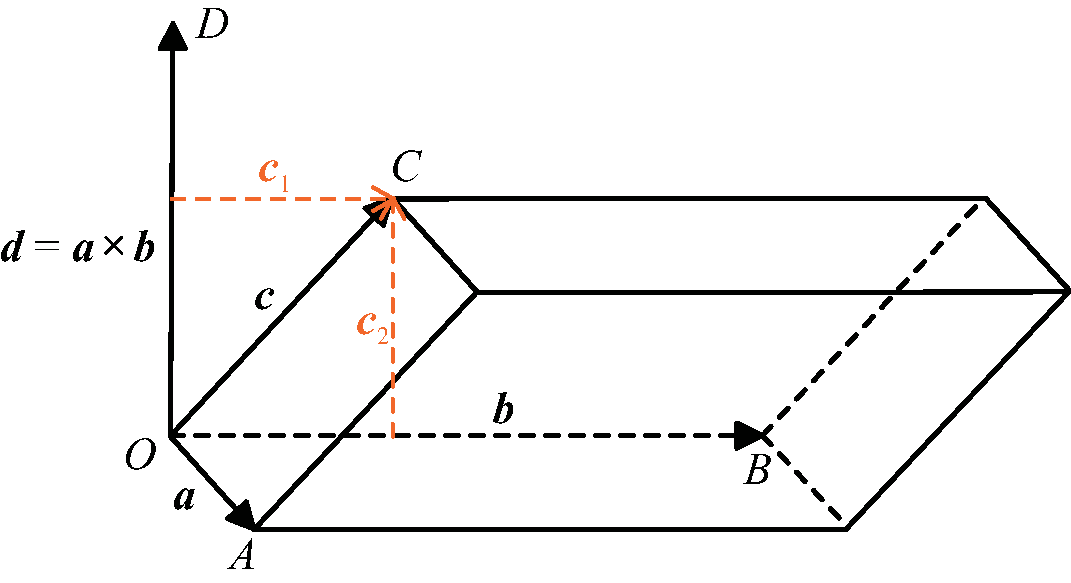
\includegraphics[width = 0.9\linewidth]{pic/C-5/vecfix}
	\vspace*{-1em}
	\captionof{figure}{向量的混合积}
	\label{向量的混合积}
\end{minipage}

\begin{equation}
	|[\boldsymbol{a}\,\boldsymbol{b}\,\boldsymbol{c}]|=(\boldsymbol{a}\times\boldsymbol{b})\cdot\boldsymbol{c}=\boldsymbol{d}\cdot\boldsymbol{c}=\boldsymbol{d}\cdot(\boldsymbol{c_1}+\boldsymbol{c_2})=\boldsymbol{d}\cdot\boldsymbol{c_2}=|\boldsymbol{d}|\cdot|\boldsymbol{c_2}|=|\boldsymbol{a}\times\boldsymbol{b}|\cdot\boldsymbol{c_2}=S_{\text{底}}\times h=V\vspace{-0.5em}
\end{equation}
也就是说混合积$[\boldsymbol{a},\boldsymbol{b},\boldsymbol{c}]$的绝对值就是这三个向量$\boldsymbol{a},\boldsymbol{b},\boldsymbol{c}$所构成的平行六面体的体积。
\vspace*{0.5em}
\\ \noindent\textbf{混合积的重要应用:}
\\ (1)$\,$求三个向量$\boldsymbol{a},\boldsymbol{b},\boldsymbol{c}$所构成的平行六面体的体积。
\\ (2)$\,$三个向量$\boldsymbol{a},\boldsymbol{b},\boldsymbol{c}$共面$\Leftrightarrow$ $[\boldsymbol{a},\boldsymbol{b},\boldsymbol{c}]=0$.
\section{向量的空间坐标}
\subsection{空间直角坐标系}
\defination[空间直角坐标系的定义]

\noindent
\begin{minipage}{0.6\linewidth}
\hspace*{2em}空间任意选定一点$O$,过点$O$作三条互相垂直的数轴$Ox,Oy,Oz$,它们都以$O$为原点且具有相同的长度单位。这三条轴分别称作$x$轴(横轴),$y$(纵轴),$z$(竖轴),统称为坐标轴。它们的正方向符合右手规则,即以右手握住$z$轴,当右手的四个手指$x$轴的正向以$90\circ$转向$y$轴正向时,大拇指的指向就是$z$轴的正向。
\hspace*{2em} 简单地讲,就是\textbf{一个原点,三个坐标轴,三个坐标面,八个卦限}。而数组$(x,y,z)$对应空间上的一点坐标。
\end{minipage}
\begin{minipage}{0.4\linewidth}
	\centering
	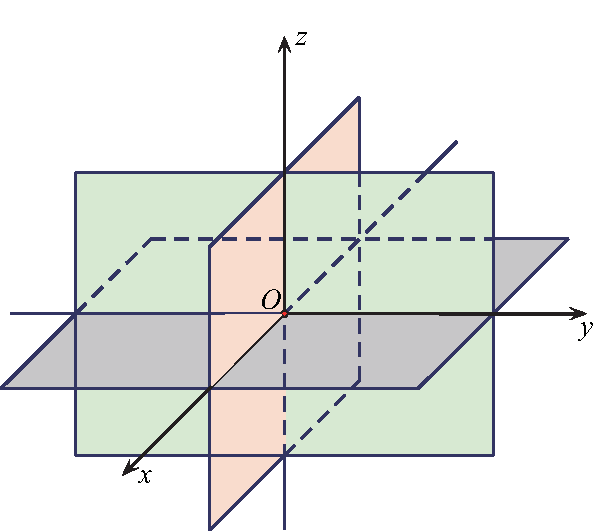
\includegraphics[width = 0.75\linewidth]{pic/C-5/空间坐标}
	\vspace*{-1em}
	\captionof{figure}{空间直角坐标系}
	\label{空间直角坐标系}
\end{minipage}

\subsection{向量的空间坐标的表示与计算}
\defination[向量的空间坐标定义]
\noindent
\begin{minipage}{0.6\linewidth}
\hspace*{2em}设向量$\boldsymbol{i},\boldsymbol{j},\boldsymbol{k}$分别为$x$轴,$y$轴,$z$轴的单位向量,那么对于空间点$A(x,y,z)$,$\boldsymbol{OA}$可以表示为
\begin{equation}
	\boldsymbol{OA}=x\boldsymbol{i}+y\boldsymbol{j}+z\boldsymbol{k}
\end{equation}
设$\boldsymbol{r}=\boldsymbol{OA}$,那么我们规定向量$\boldsymbol{r}$的坐标为$(x,y,z)$,记作$\boldsymbol{r}=(x,y,z)$.\\
1.$\,$向量的线性运算的坐标表示
\par 记向量$\boldsymbol{a}=(x_1,y_1,z_1)$,$\boldsymbol{b}=(x_2,y_2,z_2)$,那么
\end{minipage}
\begin{minipage}{0.4\linewidth}
	\centering
	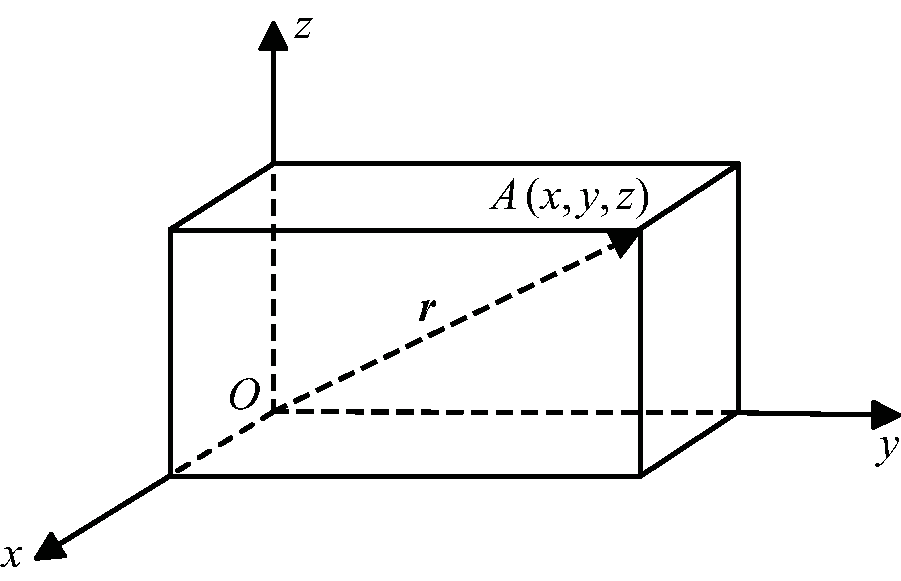
\includegraphics[width = 0.9\linewidth]{pic/C-5/veclinar}
	\vspace*{-1em}
	\captionof{figure}{向量的空间坐标表示}
	\label{向量的空间坐标表示}
\end{minipage}
\noindent(1)$\quad \boldsymbol{a}+\boldsymbol{b}=(x_1+x_2,y_1+y_2,z_1+z_2)$\\
(2)$\quad \boldsymbol{a}-\boldsymbol{b}=(x_1-x_2,y_1-y_2,z_1-z_2)$\\
(3)$\quad \lambda \boldsymbol{a}=(\lambda x_1,\lambda y_1,\lambda z_1)$\\
2.$\,$向量的内积、外积的坐标表示\\
记向量$\boldsymbol{a}=(x_1,y_1,z_1).\boldsymbol{b}=(x_2,y_2,z_2)$,那么\\
\textbf{内积:}$\boldsymbol{a}\cdot\boldsymbol{b}=x_1x_2+y_1y_2+z_1z_2$\\
特别地,$\boldsymbol{a}^2=\boldsymbol{a}\cdot\boldsymbol{a}=x_1^2+y_1^2+z_1^2$,那么向量$\boldsymbol{a}$的模长为$|\boldsymbol{a}|=\sqrt{\boldsymbol{a}^2}=\sqrt{x_1^2+y_1^2+z_1^2}$\\

\noindent 那么由$\boldsymbol{a}\cdot\boldsymbol{b}=|\boldsymbol{a}||\boldsymbol{b}|\cos\langle \boldsymbol{a},\boldsymbol{b}\rangle$,得$\di\cos\langle \boldsymbol{a},\boldsymbol{b}\rangle=\frac{\boldsymbol{a}\cdot\boldsymbol{b}}{|\boldsymbol{a}||\boldsymbol{b}|}=\frac{x_1x_2+y_1y_2+z_1z_2}{\sqrt{x_1^2+y_1^2+z_1^2}\sqrt{x_2^2+y_2^2+z_2^2}}$\\

\noindent \textbf{外积:}$\boldsymbol{a}\times\boldsymbol{b}=(y_1z_2-z_1y_2)\boldsymbol{i}+(z_1x_2-x_1z_2)\boldsymbol{j}+(x_1y_2-y_1x-2)\boldsymbol{k}=
	\begin{bmatrix}
		\boldsymbol{i} & \boldsymbol{j} & \boldsymbol{k}\\
		x_1 & y_1 & z_1\\
		x_2 & y_2 & z_2\\
	\end{bmatrix}$\\
特别地,
\begin{equation}
	\boldsymbol{a}\parallel\boldsymbol{b}\Leftrightarrow \frac{x_1}{y_1}=\frac{y_1}{y-2}=\frac{z_1}{z_2}=
\end{equation}
\textbf{混合积:}
\begin{equation}
	\nonumber
	\boldsymbol{c}\cdot(\boldsymbol{a}\times\boldsymbol{b})=(x_0\boldsymbol{i}+y_0\boldsymbol{j}+z_0\boldsymbol{k})	
	\begin{bmatrix}
		\boldsymbol{i} & \boldsymbol{j} & \boldsymbol{k}\\
		x_1 & y_1 & z_1\\
		x_2 & y_2 & z_2\\
	\end{bmatrix}=x_0\boldsymbol{i}
	\begin{bmatrix}
	\boldsymbol{i} & \boldsymbol{j} & \boldsymbol{k}\\
	x_1 & y_1 & z_1\\
	x_2 & y_2 & z_2\\
\end{bmatrix}+y_0\boldsymbol{j}	
\begin{bmatrix}
\boldsymbol{i} & \boldsymbol{j} & \boldsymbol{k}\\
x_1 & y_1 & z_1\\
x_2 & y_2 & z_2\\
\end{bmatrix}+z_0\boldsymbol{k}	
\begin{bmatrix}
\boldsymbol{i} & \boldsymbol{j} & \boldsymbol{k}\\
x_1 & y_1 & z_1\\
x_2 & y_2 & z_2\\
\end{bmatrix}
\end{equation}
\begin{equation}
	\nonumber
	=\begin{bmatrix}
		x_0\boldsymbol{i}\cdot\boldsymbol{i} & x_0\boldsymbol{i}\cdot\boldsymbol{j} & x_0\boldsymbol{i}\cdot\boldsymbol{k}\\
	x_1 & y_1 & z_1\\
	x_2 & y_2 & z_2\\
	\end{bmatrix}+
\begin{bmatrix}
	y_0\boldsymbol{j}\cdot\boldsymbol{i} & y_0\boldsymbol{j}\cdot\boldsymbol{j} & y_0\boldsymbol{j}\cdot\boldsymbol{k}\\
	x_1 & y_1 & z_1\\
	x_2 & y_2 & z_2\\
\end{bmatrix}+
\begin{bmatrix}
	z_0\boldsymbol{k}\cdot\boldsymbol{i} & z_0\boldsymbol{k}\cdot\boldsymbol{j} & z_0\boldsymbol{k}\cdot\boldsymbol{k}\\
	x_1 & y_1 & z_1\\
	x_2 & y_2 & z_2\\
\end{bmatrix}=
\begin{bmatrix}
	x_0 & y_0 & z_0\\
	x_1 & y_1 & z_1\\
	x_2 & y_2 & z_2\\
\end{bmatrix}
\end{equation}
(注:$\boldsymbol{i}\cdot\boldsymbol{i}=1,\boldsymbol{i}\cdot\boldsymbol{j}=0,\boldsymbol{i}\cdot\boldsymbol{k}=0$其余类似可得,本质上就是利用三个坐标轴上的单位向量相乘)
\subsection{方向角与方向余弦}
\defination[方向角与方向余弦]
\vspace*{0.5em}
\noindent
\begin{minipage}{0.6\linewidth}
\hspace*{2em}记非零向量$\boldsymbol{r}$与三条坐标轴$(x,y,z)$的夹角$\alpha,\beta,\gamma$为向量$\boldsymbol{r}$的方向角。设$\boldsymbol{r}=\boldsymbol{OA}=(x,y,z)$,则
\begin{equation}
	\cos \alpha=\frac{x}{|OA|}=\frac{x}{\boldsymbol{|r|}}=\frac{x}{\sqrt{x^2+y^2+z^2}}
\end{equation}
\begin{equation}
	\cos \beta=\frac{y}{|OA|}=\frac{y}{\boldsymbol{|r|}}=\frac{y}{\sqrt{x^2+y^2+z^2}}
\end{equation}
\begin{equation}
	\cos \gamma=\frac{z}{|OA|}=\frac{z}{\boldsymbol{|r|}}=\frac{z}{\sqrt{x^2+y^2+z^2}}
\end{equation}
那么,向量$\boldsymbol{r}$方向上的方向向量可以表示成:
\end{minipage}
\begin{minipage}{0.4\linewidth}
	\centering
	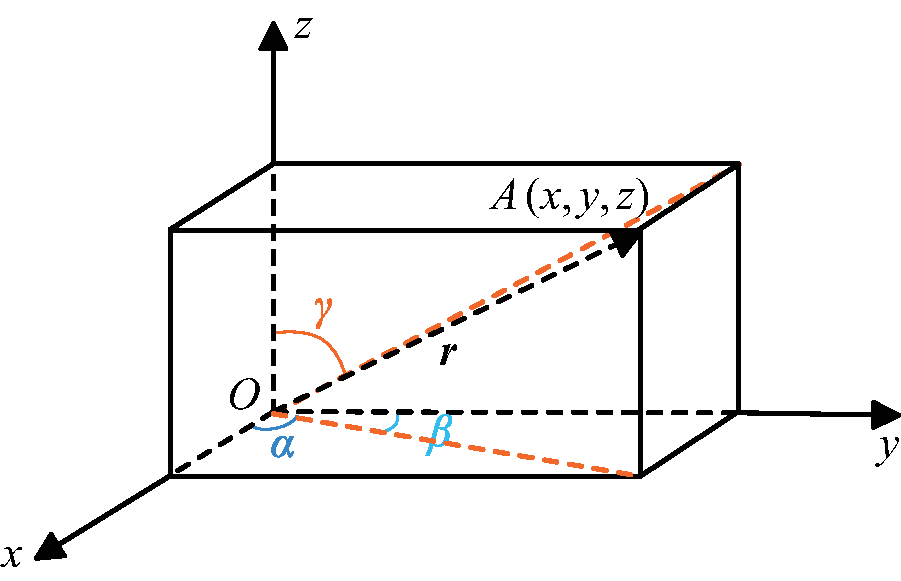
\includegraphics[width = 0.85\linewidth]{pic/C-5/vesang3}
	\vspace*{-1em}
	\captionof{figure}{向量的方向角}
	\label{向量的方向角}
\end{minipage}

\begin{equation}
	\boldsymbol{e_r}=(\cos \alpha,\cos \beta,\cos \gamma)=\bigg(\frac{x}{|\boldsymbol{r}|},\frac{y}{|\boldsymbol{r}|},\frac{z}{|\boldsymbol{r}|}\bigg)=\frac{1}{|\boldsymbol{r}|}(x,y,z)=\frac{\boldsymbol{r}}{|\boldsymbol{r}|}
\end{equation}
\section{空间平面与空间直线}
\subsection{平面的方程}
平面的方程一般有四种表达方式:点法式、一般式、三点式、截距式。
\\ 

\noindent
\begin{minipage}{0.6\linewidth}
1.$\,$平面的点法式方程\\ 
\hspace*{2em}设平面的法向量$\boldsymbol{n}$(即垂直于平面的向量)的坐标为(A,B,C(A,B,C不全为0))。设点$P_0(x_0,y_0,z_0)$在平面上,那么平面上任意一点$P(x,y,z)$满足:
\begin{equation}
	\nonumber
	\boldsymbol{n}\cdot\boldsymbol{PP_0}=0
\end{equation}
即\begin{equation}
	A(x-x_0)+B(y-y_0)+C(z-z_0)=0
	\end{equation}
\vspace*{0.1em}
\end{minipage}
\begin{minipage}{0.4\linewidth}
	\centering
	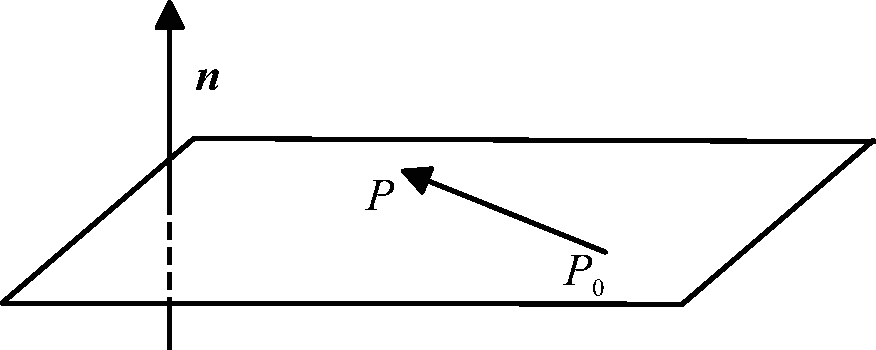
\includegraphics[width = 0.9\linewidth]{pic/C-5/plane1}
	\vspace*{-1em}
	\captionof{figure}{平面的点法式方程}
	\label{平面的点法式方程}
\end{minipage}

同样地,如果空间中任何一点$P(x,y,z)$满足这个方程,那么这个点一定在平面上。
\\这个方程是由平面的一个法向量及平面上一已知点的坐标确定的,故通常称为\highlight{dy}{\index{PMDDFSFC@平面的点法式方程}平面的点法式方程}。\\
2.$\,$平面的一般式方程
\par 我们将点法式方程进一步化简,得:
\begin{equation}
	A(x-x_0)+B(y-y_0)+C(z-z_0)=0\Leftrightarrow Ax+By+Cz-Ax_0-By_0-Cz_0=0
	\label{equ:5.16}
\end{equation}
设式\eqref{equ:5.16}中,$D=-Ax_0-By_0-Cz_0$.上式变为:
\begin{equation}
	Ax+By+Cz+D=0
\end{equation}
那么,式\ref{equ:5.16}称为\highlight{dy}{\index{PMDYBSFC@平面的一般式方程}平面的一般式方程}。\\

\noindent
\begin{minipage}{0.6\linewidth}
3.$\,$平面的三点式方程\\
\hspace*{2em}已知平面上的三点$P_1(x_1,y_1,z_1),P_2(x_2,y_2,z_2),P_3(x_3,y_3,z_3)$,要使这三点能够唯一地确定一个平面,那么这三个点必然不共线。即$\boldsymbol{P_1P_2}\times\boldsymbol{P_1P_3}\neq 0$。那么,平面上任意一点必满足:
\begin{equation}
	\boldsymbol{P_1P}\cdot(\boldsymbol{P_1P_2}\times\boldsymbol{P_1P_3})=0
\end{equation}
\end{minipage}
\begin{minipage}{0.4\linewidth}
	\centering
	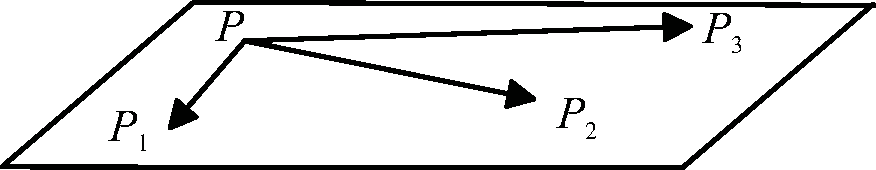
\includegraphics[width = 0.85\linewidth]{pic/C-5/plane2}
	\vspace*{-1em}
	\captionof{figure}{平面的三点式方程}
	\label{平面的三点式方程}
\end{minipage}

\noindent 即\begin{equation}
	\boldsymbol{P_1P}\cdot(\boldsymbol{P_1P_2}\times\boldsymbol{P_1P_3})=(x-x_1,y-y_1,z-z_1)\cdot
	\begin{vmatrix}
		\boldsymbol{i} & \boldsymbol{j} & \boldsymbol{k}\\
		x_2-x_1 & y_2-y_1 & z_2-z_1\\
		x_3-x_1 & y_3-y_1 & z_3-z_1\\
	\end{vmatrix}=
\begin{vmatrix}
	x-x_1 & y-y_1 & z-z_1\\
	x_2-x_1 & y_2-y_1 & z_2-z_1\\
	x_3-x_1 & y_3-y_1 & z_3-z_1\\
\end{vmatrix}=0
\end{equation}
即\begin{equation}
	\begin{vmatrix}
		x-x_1 & y-y_1 & z-z_1\\
		x_2-x_1 & y_2-y_1 & z_2-z_1\\
		x_3-x_1 & y_3-y_1 & z_3-z_1\\
	\end{vmatrix}=0
\label{equ:5-20}
\end{equation}
那么,式\eqref{equ:5-20}称为\highlight{dy}{\index{PMDSDSFC@平面的三点式方程}平面的三点式方程}。\\
4.$\,$平面的截距式方程
\par 我们将平面的一般方程$Ax+By+Cz+D=0$进一步变形,当$A,B,C,D\neq0$时,两边同时除以$-D$,得
\begin{equation}
	\displaystyle \frac{x}{-\frac{D}{A}}+\frac{y}{-\frac{D}{B}}+\frac{z}{-\frac{D}{C}}
=1\end{equation}
这个方程称为\highlight{dy}{\index{PMDJJSFC@平面的截距式方程}平面的截距式方程}。从中也比较容易看出平面与截距的关系。\\

\vspace*{-1em}
\noindent
\begin{minipage}{0.6\linewidth}
当$D=0$时,说明平面一定过原点。\\
当$A=0$时,平面$By+Cz+D=0$与$x$轴平行。\\
当$B=0$时,平面$Ax+Cz+D=0$与$y$轴平行。\\
当$C=0$时,平面$Ax+By+D=0$与$z$轴平行。\\
当$A,B=0$时,平面$Cz+D=0$与平面$Oxy$轴平行。\\
当$B,C=0$时,平面$Ax=0$与平面$Oyz$轴平行。\\
当$A,C=0$时,平面$By=0$与平面$Oxz$轴平行。\\
\end{minipage}
\begin{minipage}{0.4\linewidth}
	\centering
	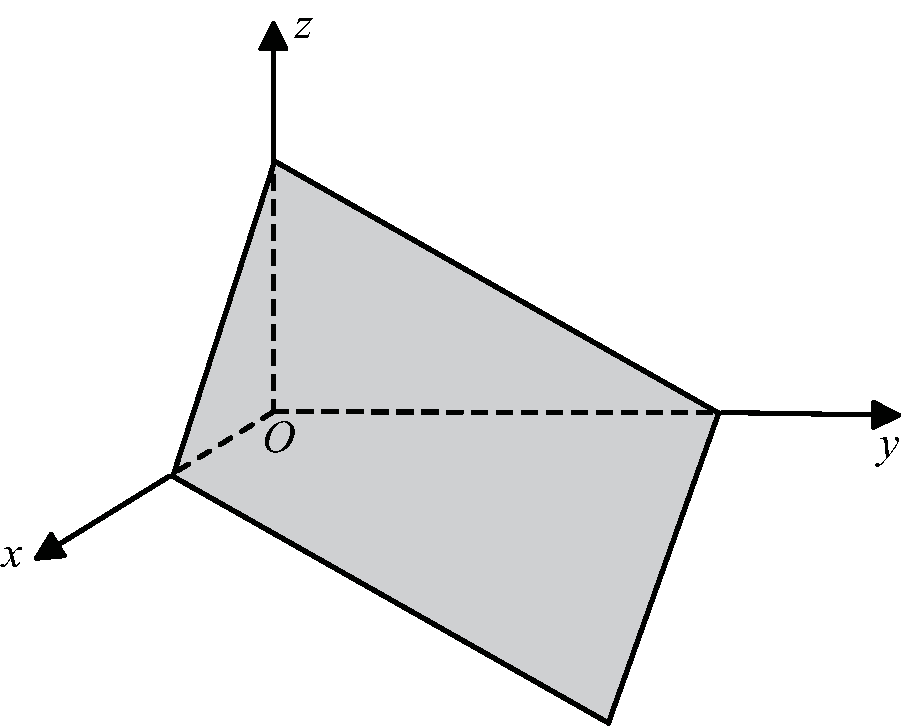
\includegraphics[width = 0.8\linewidth]{pic/C-5/plane3}
	\vspace*{-1em}
	\captionof{figure}{平面的截距式方程}
	\label{平面的截距式方程}
\end{minipage}
5.$\,$平面的方程总结
\par 我们通过对比二维直线的表达式和三维平面的表达式来更好地理解和记忆三维平面方程。
\begin{table}[h]
	\centering
	\setlength{\tabcolsep}{10mm}{
	\begin{tabular}{ccc}
		\toprule[1.5pt]
		方程类型 & 二维直线表达式 & 三维平面表达式\\
		\midrule[0.7pt]
		点法式 & $A(x-x_0)+B(y-y_0)=0$ & $A(x-x_0)+B(y-y_0)+C(z-z_0)=0$\\[0.5em]
		一般式 & $Ax+By+C=0$ & $Ax+By+Cz+D=0$\\[0.5em]
		截距式 & $\displaystyle \frac{x}{a}+\frac{y}{b}=1$ & $\displaystyle \frac{x}{  -\frac{D}{A}}+\frac{y}{-\frac{D}{B}}+\frac{z}{-\frac{D}{C}}=1$\\[1em]
		(两)三点式 & $\displaystyle y=kx+b,k=\frac{y_2-y_1}{x_2-x_1}$ & $\begin{vmatrix}
				x-x_1 & y-y_1 & z-z_1\\
			x_2-x_1 & y_2-y_1 & z_2-z_1\\
			x_3-x_1 & y_3-y_1 & z_3-z_1\\
		\end{vmatrix}=0$\\
		\bottomrule[1.5pt]
	\end{tabular}
}
\end{table}
\subsection{直线的方程}
直线的方程一般有三种表示方式:一般方程(两面式)、参数方程、标准方程。\\
1.$\,$直线的点法式方程
\par 在空间中,直线一般是由两个平面相交而得到的交线,因此,直线可以用两个平面的方程联立得到。\\

\noindent
\begin{minipage}{0.6\linewidth}
 设两个相交平面为:
\begin{equation}
	\nonumber
	\Pi_1:A_1x+B_1y+C_1z+D_1=0
\end{equation}
\begin{equation}
	\nonumber
\Pi_2: A_2x+B_2y+C_2z+D_2=0
\end{equation}
联立得,
\begin{equation}
	L:\begin{cases}
	\, A_1x+B_1y+C_1z+D_1=0\\
	\, 	A_2x+B_2y+C_2z+D_2=0\\
		\end{cases}
	\label{equ:5.22}
\end{equation}
那么式\eqref{equ:5.22}就称为\highlight{dy}{\index{ZXDLMDFCHYBFC@直线的两面式方程或一般方程}直线的两面式方程或一般方程}。
\vspace*{0.5em}
\end{minipage}
\begin{minipage}{0.4\linewidth}
	\centering
	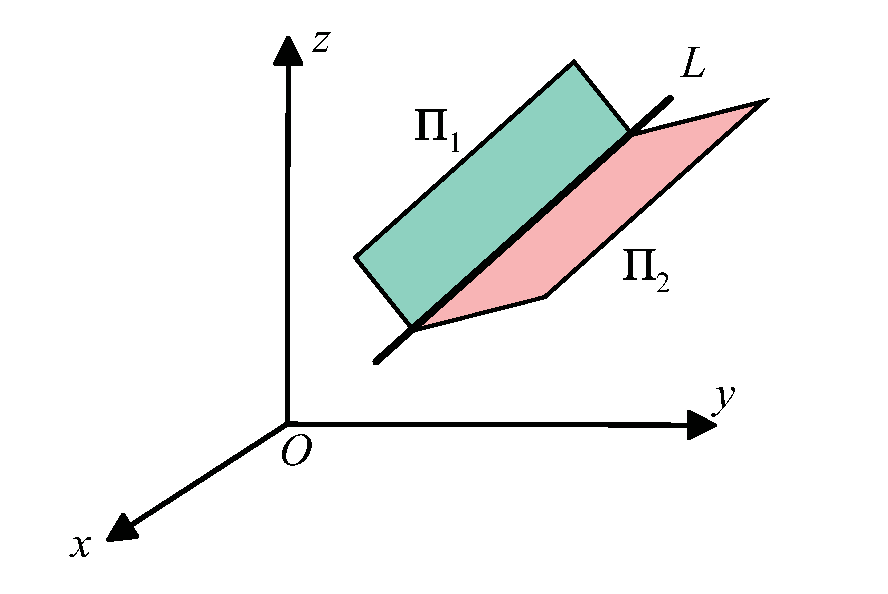
\includegraphics[width = 0.85\linewidth]{pic/C-5/line}
	\vspace*{-1em}
	\captionof{figure}{向量的点法式方程}
	\label{直线的点法式方程}
\end{minipage}

\noindent 2.$\,$直线的参数方程
\par 已知直线的一点$P_0(x_0,y_0,z_0)$,且直线的非零方向向量为$\boldsymbol{e}=(a,b,c)$,那么就存在一个实数$t$,使得直线上任意一点$P$都满足:
\begin{equation}
	\boldsymbol{P_0P}=t\boldsymbol{e}(-\infty<t<+\infty)
\end{equation}
即
\begin{equation}
	\begin{cases}
		\, x-x_0=ta\\
		\, y-y_0-tb\\
		\, z-z_0=tc
	\end{cases}
(-\infty<t<+\infty)
\label{equ:5.23}
\end{equation}
那么式\eqref{equ:5.23}就称为\highlight{dy}{\index{ZXDCSFC@直线的参数方程}直线的参数方程}。
\\ 3.$\,$直线的标准方程
\par 在直线的参数方程ref{equ:5.23}的基础上进一步消去参数,得
\begin{equation}
	\frac{x-x_1}{a}=\frac{y-y_1}{b}=\frac{z-z_1}{c}
\label{equ:5.24}
\end{equation}
那么式\eqref{equ:5.24}就称为\highlight{dy}{\index{ZXDBZFC@直线的标准方程}直线的标准方程}。上述的写法只是一个形式上的写法,实际上完整的式子应该为:
\begin{equation}
	\begin{cases}
		\, a(y-y_0)-b(x-x_0)=0\\
		\, a(z-z_0)-c(x-x_0)=0\\
	\end{cases}
\end{equation}
这时就不需要对$a,b,c$是不是0进行分类讨论。
\\ 4*.$\,$平面束方程
\par 设直线$L$由方程组:
\begin{equation}
	\begin{cases}
\, A_1x+B_1y+C_1z+D_1=0\\
\, A_2x+B_2y+C_2z+D_2=0\\
\end{cases}
\end{equation}
确定。其中$A_1,B_1,C_1$与$A_2,B_2,C_2$不成比例。(目的是使两个平面不平行)那么我们建立三元一次方程
\begin{equation}
	A_1x+B_1y+C_1z+D_1+\lambda(A_2x+B_2y+C_2z)+D_2=0
\label{equ:5-41}	
\end{equation}
其中$\lambda$为任意常数。进一步化简,可得
\begin{equation}
	(A_1+\lambda A_1)x+(B_1+\lambda B_2)y+(C_1+\lambda C_2Z)+(D_1+D_2)=0
\end{equation}
\par 由于$A_1,B-1,C_1$与$A_2,B_2,C_2$不成比例,$(A_1+\lambda A_1),(B_1+\lambda B_2),(C_1+\lambda C_2Z),(D_1+D_2)$都部为0.那么上述方程代表的就是一个平面,而由于$\lambda$不确定,而且直线$L$必定是这个方程的解,那么方程\eqref{equ:5-41}就代表着所有通过定直线$L$的平面,称为通过直线$L$的\highlight{dy}{\index{PMSDFC@平面束的方程}平面束的方程}。

\noindent
\begin{minipage}{0.6\linewidth}
\subsection{平面与直线的夹角问题}
1.$\,$平面与平面的夹角
\par 已知两个平面$\Pi_1,\Pi_2$:
\begin{equation}
	\nonumber
	\Pi_1:A_1x+B_1y+C_1z+D_1=0
\end{equation}
\begin{equation}
	\nonumber
	\Pi_2: A_2x+B_2y+C_2z+D_2=0
	\end{equation}
\end{minipage}
\begin{minipage}{0.4\linewidth}
	\centering
	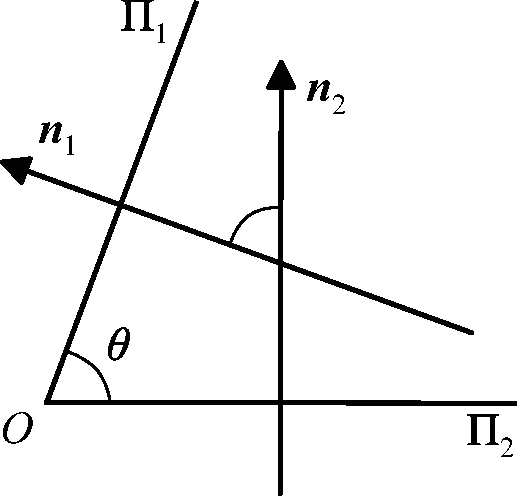
\includegraphics[width = 0.65\linewidth]{pic/C-5/planeang}
	\vspace*{-1em}
	\captionof{figure}{平面与平面的夹角}
	\label{平面与皮昂面的夹角}
\end{minipage}

\noindent 那么它们的夹角$\theta$的余弦值为:
\begin{equation}
	\cos \theta=\cos\langle \boldsymbol{n_1},\boldsymbol{n_2}\rangle =\frac{\boldsymbol{n_1}\cdot\boldsymbol{n_2}}{|\boldsymbol{n_1}||\boldsymbol{n_2}|}=\frac{|A_1A_2+B_1B_2+C_1C_2|}{\sqrt{A_1^2+B_1^2+C_1^2}\cdot\sqrt{A_2^2+B_2^2+C_2^2}}
\end{equation}
那么,我们可以通过这个式子来判断平面之间的关系:\\
(1)$\, \Pi_1\perp \Pi_2 \Leftrightarrow  A_1A_2+B_1B_2+C_1C_2=0$\\

\noindent
\begin{minipage}{0.7\linewidth}
(2)$\, \Pi_1\parallel \Pi_2 \Leftrightarrow \displaystyle \frac{A_1}{A_2}=\frac{B_1}{B_2}=\frac{C_1}{C_2} $\vspace*{-0.5em}\\

2.$\,$直线与直线的夹角
\par 已知两条直线$L_1,L_2$:
\begin{equation}
	L_1: \frac{x-x_1}{m_1}=\frac{y-y_1}{n_1}=\frac{z-z_1}{p_1}
\end{equation}
\begin{equation}
	L_2:\frac{x-x_2}{m_2}=\frac{y-y_2}{n_2}=\frac{z-z_2}{p_2}
\end{equation}
那么它们的夹角$\theta$的余弦值为:
\end{minipage}
\begin{minipage}{0.35\linewidth}
	\centering
	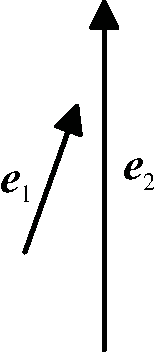
\includegraphics[width = 0.3\linewidth]{pic/C-5/lineang}
	\vspace*{-1em}
	\captionof{figure}{直线与直线的夹角}
	\label{直线与直线的夹角}
\end{minipage}

\begin{equation}
\cos\langle L_1,L_2\rangle =\cos \langle \boldsymbol{e_1},\boldsymbol{e_2}\rangle =\frac{\boldsymbol{e_1}\cdot\boldsymbol{e_2}}{|\boldsymbol{e_1}||\boldsymbol{e_2}|}=\frac{|m_1m_2+n_1n_2+p_1p_2|}{\sqrt{m_1^2+n_1^2+p_1^2}\sqrt{m_2^2+n_2^2+p_2^2}}
\end{equation}
那么,我们可以通过这个式子来判断直线之间的关系:\\
(1)$\, L_1\perp L_2 \Leftrightarrow  m_1m_2+n_1n_2+p_1p_2=0$\\
(2)$\, L_1\parallel L_2 \Leftrightarrow \displaystyle \frac{m_1}{m_2}=\frac{n_1}{n_2}=\frac{p_1}{p_2} $\\

\noindent
\begin{minipage}{0.7\linewidth}
3.$\,$直线与平面的夹角
\par 已知直线$L$和平面$\Pi$:
\begin{equation}
	\nonumber
	L:\frac{x-x_0}{m}=\frac{y-y_0}{n}=\frac{z-z_0}{p}
\end{equation}
\begin{equation}
	\nonumber
	\Pi:Ax+By+Cz+D=0
\end{equation}
那么它们的夹角$\theta$的正弦值为:
\end{minipage}
\begin{minipage}{0.3\linewidth}
	\centering
	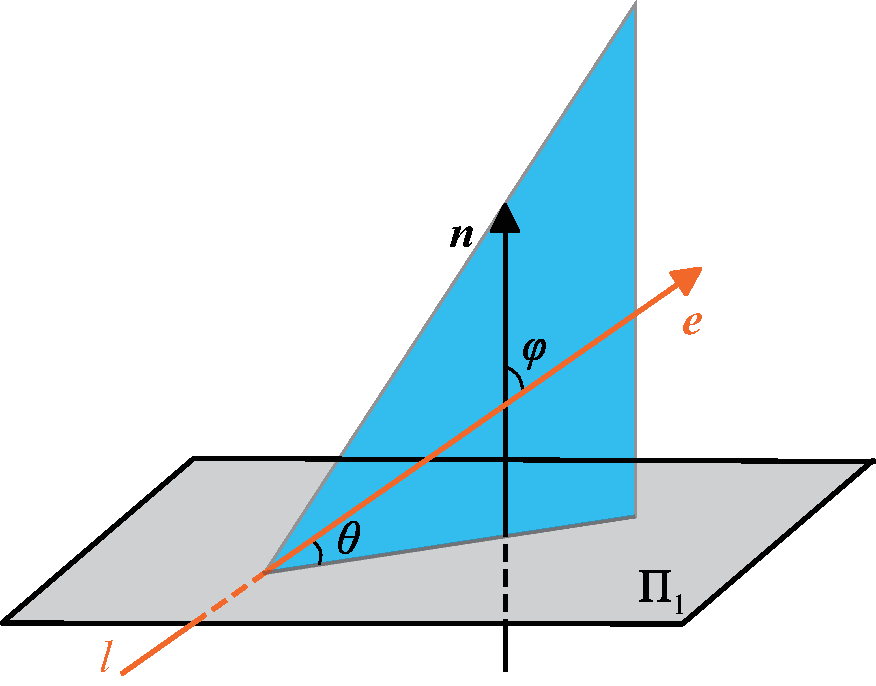
\includegraphics[width = 0.95\linewidth]{pic/C-5/planelineang}
	\vspace*{-1em}
	\captionof{figure}{直线与平面的夹角}
	\label{直线与平面的夹角}
\end{minipage}

\begin{equation}
	\sin \varphi =\cos\bigg( \frac{\pi}{2}-\varphi\bigg)=\cos \theta=\cos \langle \boldsymbol{e},\boldsymbol{n}\rangle =\frac{|Am+Bn+Cp|}{\sqrt{A^2+B^2+C^2}\cdot\sqrt{m^2+n^2+p^2}}
\end{equation}
那么,我们可以通过这个式子来判断直线与平面之间的关系:\\
(1)$\, L\perp \Pi \Leftrightarrow  Am+Bn+Cp=0$\\
(2)$\, L\parallel \Pi \Leftrightarrow \displaystyle \frac{A}{m}=\frac{B}{n}=\frac{C}{p} $
\subsection{平面与直线的距离问题}
\noindent 1.$\,$点与点的距离
\par 设点$M_1(x_1,y_1,z_1),M_2(x_2,y_2,z_2)$,那么两点间距离
\begin{equation}
	|M_1M_2|=\sqrt{(x_2-x_1)^2+(y_2-y_1)^2+(z_2-z_1)^2}
\end{equation}
2.$\,$点到平面的距离
\par 已知一个平面$Ax+By+Cz+D=0(A,B,C$不全为0)和平面外一点$P_1(x_1,y_1,z_1)$,取平面内一点$P_0(x_0,y_0,z_0)$,那么点$P_1$到平面的距离为:
\begin{equation}
	d=|\boldsymbol{P_0P_1}|\cos \langle \boldsymbol{P_0P_1}\cdot \boldsymbol{n} \rangle|=\frac{\boldsymbol{P_0P_1}\cdot \boldsymbol{n}}{\boldsymbol{n}}=\frac{|A(x_1-x_0)+B(y_1-y_0)+C(z_1-z_0)|}{\sqrt{A^2+B^2+C^2}}
\end{equation}

\noindent
\begin{minipage}{0.7\linewidth}
又$P_0$在平面$Ax+By+Cz+D=0$上,\\
所以,$D=-Ax_0-By_0-Cz_0$,即
\end{minipage}
\begin{minipage}{0.3\linewidth}
	\centering
	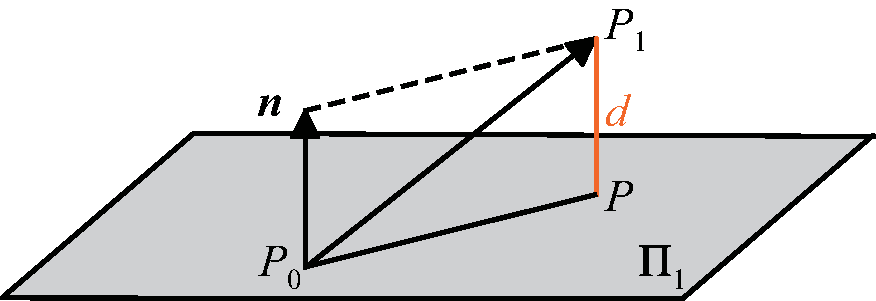
\includegraphics[width = 0.9\linewidth]{pic/C-5/planed}
	\vspace*{-1em}
	\captionof{figure}{点到平面的距离}
	\label{点到平面的距离}
\end{minipage}

\begin{equation}
	d=\frac{|A(x_1-x_0)+B(y_1-y_0)+C(z_1-z_0)|}{\sqrt{A^2+B^2+C^2}}=\frac{|Ax_1+By_1+Cz_1+D|}{\sqrt{A^2+B^2+C^2}}
\end{equation}
\vspace*{-2.5em}
\summarize[\hspace*{2em}联想二维空间中点到直线的距离公式进行记忆:
\begin{equation}
	d=\frac{|Ax_1+By_1+C|}{\sqrt{A^2+B^2}}
	\end{equation}]

\noindent
\begin{minipage}{0.7\linewidth}\noindent 
	3.$\,$直线到平面的距离/平面到平面的距离
	\hspace*{2em} 我们只需要在直线或者平面上任取一个点,就变成点到平面的距离问题。\\
	4.$\,$点到直线的距离
 \\ \hspace*{2em} 已知一条直线
\begin{equation}
	L:\frac{x-x_0}{m}=\frac{y-y_0}{n}=\frac{z-z_0}{p}
\end{equation}
和直线外一点$P_1(x_1,y_1,z_1)$,过点$P_1$作平面垂直于直线$L$,交于点$P$,那么平面的方程为:
\begin{equation}
	m(x-x_1)+n(y-y_1)+p(z-z_1)=0
\end{equation}
\end{minipage}
\begin{minipage}{0.4\linewidth}
	\centering
	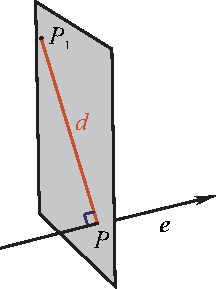
\includegraphics[width = 0.5\linewidth]{pic/C-5/linepd}
	\vspace*{-1em}
	\captionof{figure}{点到空间直线的距离}
	\label{点到空间直线的距离}
\end{minipage}

\vspace*{0.5em}
\noindent 那么联立平面与直线方程,得
\begin{equation}
	\begin{cases}
		\, m(x-x_1)+n(y-y_1)+p(z-z_1)=0\\
		\, m(y-y_0)-n(x-x_0)=0\\
		\, m(z-z_0)-p(x-x_0)=0\\
	\end{cases}
\end{equation}
然后解出$P$点的坐标,用两点间的距离公式计算出$d$的值。
\\ 5.$\,$平行直线的距离
\par 我们只需要在任意一条直线上任取一个点,就变成点到直线的距离问题。
\section{空间曲面}
\subsection{旋转曲面}

\defination[旋转曲面]

\noindent
\begin{minipage}{0.65\linewidth}
\hspace*{2em}以一条平面曲线绕其平面上的一条直线旋转一周所成的曲面叫做\highlight{dy}{\index{XZQM@旋转曲面}旋转曲面},旋转曲线和定直线依次叫做旋转曲面的\highlight{dy}{\index{MX@母线}母线}和\highlight{dy}{\index{Z@轴}轴}。
\hspace*{2em} 设在$yOz$坐标面上有一已知曲面$C$,它的方程为
\begin{equation}
	f(y,z)=0
\end{equation}
把这条曲线绕$z$轴旋转一周,就得到一个以$z$轴为旋转轴的旋转曲面,它的方程可以用以下的方法求解。\\
设$P_0(0,y_0,z_0)$为曲线$C$上任意一点,则有
\begin{equation}
	f(y_0,z_0)=0
\end{equation}
\end{minipage}
\begin{minipage}{0.35\linewidth}
	\centering
	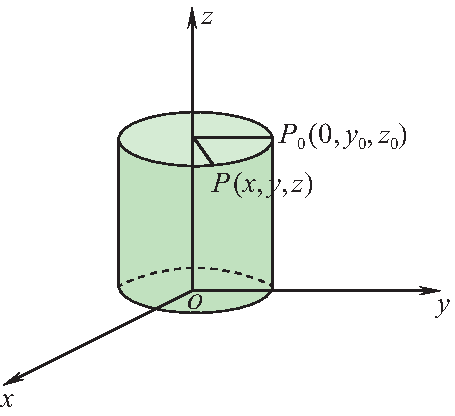
\includegraphics[width = 0.9\linewidth]{pic/C-5/yz}
	\vspace*{-1em}
	\captionof{figure}{旋转曲面}
	\label{旋转曲面}
\end{minipage}

\vspace*{0.5em}
\noindent 当曲线$C$绕$z$轴旋转时,$P_0(0,y_0,z_0)$旋转为$P(x,y,z)$,利用旋转前后点到$z$轴的距离不变,我们可以得到$x,y,z$与$y_0,z_0$的对应关系如下:
\begin{equation}
	\begin{cases}
	\,  d=y_0=\pm\sqrt{x^2+y^2}\\
	\, z_0=z\\
	\end{cases}
\end{equation}
又$f(y_0,z_0)=0$,所以旋转后的曲面方程为:
\begin{equation}
	f(\pm\sqrt{x^2+y^2},z)=0
\end{equation}
同理可得,曲线$C$绕$y$轴旋转所得到的曲面方程为
\begin{equation}
	f(y,\pm \sqrt{x^2+z^2})=0
\end{equation}
\subsection{柱面}

\defination[柱面]

\noindent
\begin{minipage}{0.65\linewidth}
\hspace*{2em}一般地,直线$L$沿定曲线$C$平行移动形成的轨迹叫做\highlight{dy}{\index{ZM@柱面}柱面},定曲线$C$叫做柱面的\highlight{dy}{\index{ZX@准线}准线},动直线$L$叫做柱面的\highlight{dy}{\index{MX@母线}母线}。\\
\hspace*{2em} 一般地,只含$x,y$而缺$z$的方程$F(x,y)=0$在空间直角坐标系中表示母线平行于$z$轴的柱面,其准线是$xOy$面上的曲线$C$:$F(x,y)=0$.\\
\hspace*{2em} 类似可知,只含$x,z$而缺$y$的方程$G(x,z)=0$和只含$y,z$而缺$x$的方程$H(y,z)=0$分别表示母线平行于$y$轴和$x$轴的柱面。
\end{minipage}
\begin{minipage}{0.35\linewidth}
	\centering
	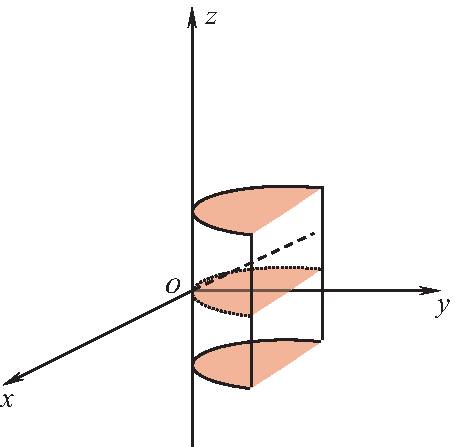
\includegraphics[width = 0.85\linewidth]{pic/C-5/zhuti}
	\vspace*{-1em}
	\captionof{figure}{柱面}
	\label{柱面}
\end{minipage}